\newpage
\thispagestyle{empty}
\section{Einleitung Neuronale Netze}\label{sec:einleitung_nn}   

\vspace{1cm}

\begin{tcolorbox}[title={Inhalt}]
  \begin{quotation}\noindent
      Dieses Kapitel liefert einen Einstieg in neuronale Netze. Es werden an Beispielen unterschiedliche Anwendungsfälle anschaulich gemacht.
      Ebenso soll bereits eine grobe Idee näher gebracht werden, wie ein neuronales Netz aufgebaut ist.
      Insgesamt werden in diesem Kapitel bereits zahlreiche grundlegende Begriffe erklärt, die in den nachfolgenden Kapiteln benötigt werden.
  \end{quotation}
  \begin{itemize}  
    \item Wofür benötigt man Neuronale Netze?
    \item Einsatzgebiete
    \item Grobes Prinzip
  \end{itemize}
\end{tcolorbox}

\subsection{Wofür benötigt man Neuronale Netze?}\label{subsec:einleitung_nn:wofuer_nn}
Mit neuronalen Netzen lassen sich Probleme lösen, die mit herkömmlichen Algorithmen nur schwer bis gar nicht lösbar sind. Neuronale Netze sind grundsätzlich in der Lage, nichtlineare Abbildungen anzunähern, Beispiele folgen weiter unten (siehe \ref*{subsec:einleitung_nn:einsatzgebiete}).
Der große Vorteil neuronaler Netze liegt darin, dass sie selbstständig lernen können, Muster in Daten zu erkennen, wodurch man die entsprechenden Algorithmen nicht mehr von Hand schreiben muss.
Neuronale Netze sind dabei in der Lage, auch komplexe Muster und Zusammenhänge aus sehr großen Datenmengen zu erkennen und zu extrahieren.

\bigbreak\noindent
Aufgrund ihrer Fähigkeit, schnell und effizient komplexe Muster zu erkennen, können neuronale Netze auch Aufgaben lösen, für die man normalerweise Menschen benötigen würde, da herkömmliche Algorithmen diese Probleme nicht zuverlässig genug lösen können oder der Entwicklungsaufwand unverhältnismäßig groß in Relation zum Nutzen wäre.

\bigbreak\noindent
Häufig sind Muster zu komplex, um sie mit einem klassischen Algorithmus erfassen zu können oder sie sind schlecht von Hand mathematisch formulierbar.
Ein Beispiel hierfür wäre die Erkennung von Tieren auf einem Foto. Die Eigenschaften, die z.B. eine Katze ausmachen von Hand in Bedingungen zu überführen ist nahezu unmöglich, gerade deswegen da die Katzen sehr verschieden aussehen können und aus verschiedenen Perspektiven auf dem Foto zu sehen sein können und die Menge an Merkmalen viel zu groß und komplex ist.
Mit Hilfe eines neuronalen Netzes kann man aber dennoch mit relativ geringem Aufwand ein Netz trainieren, das in der Lage ist, solche Bilderkennungsaufgaben zu erledigen.

\bigbreak\noindent
Neuronale Netze sind häufig auch zuverlässiger bei der Lösung eines Problems, als klassische Algorithmen, da herkömmliche Algorithmen manchmal bestimmte Sonderfälle nicht abdecken können, wohingegen neuronale Netze anpassungsfähiger sind und teilweise mit solchen Sonderfällen umgehen können, da sie diese Fälle aus ihren Trainingsdaten extrahieren konnten, ein menschlicher Entwickler diese aber bei der Entwicklung eines Algorithmus übersehen hätte.
Ein Beispiel für solche Fälle könnten autonom fahrende Fahrzeuge sein.
Bei diesen ist es schwer möglich, Algorithmen zu schreiben, die unter allen Wetter-, Straßen- und Umweltbedingungen zuverlässig funktionieren.
Schlecht zu sehende Straßenschilder oder Straßen mit undeutlichen Markierungen könnten ein Problem für solche Algorithmen darstellen, da handgeschriebene Algorithmen meistens auf genau solche Straßenmerkmale angewiesen sind.
Neuronale Netze hingegen können möglicherweise mit solchen Fällen umgehen könnten, da sie sich aus den Trainingsdaten mehrere Faktoren abgeleitet haben, an denen sie sich orientieren können und zuverlässiger in der Erkennung von Mustern wie Straßenschildern sind.

\subsection{Einsatzgebiete}\label{subsec:einleitung_nn:einsatzgebiete}
Neuronale Netze sind äußerst vielfältig und lassen sich für verschiedenste Anwendungen anpassen und trainieren.
Zu den häufigsten Anwendungsfällen zählen die Bilderkennung und die Verarbeitung von auditiven Daten.

\bigbreak\noindent
Die Bilderkennung mittels neuronaler Netze lässt sich beispielsweise dazu einsetzen, medizinische Diagnosen durchzuführen, da diese Netze fähig sind, komplexe Krankheitsbilder zu erkennen.
Röntgenbilder können von neuronalen Netzen auf Anzeichen von Tumoren untersucht werden und können so medizinisches Fachpersonal bei Ihrer Arbeit unterstützen.
Auch kann die Bilderkennung genutzt werden, um die Position von Personen oder anderen Objekten auf einem Kamerabild zu identifizieren, was zur Realisierung von autonomem Fahren nützlich ist.
Dabei werden vor allem sogenannte “convolutional neural networks” verwendet.
Dabei handelt es sich um eine Variante von neuronalen Netzen, die auf Grund der speziellen verwendeten Schichten und Aktivierungsfunktionen besonders gut für die Bilderkennung geeignet sind.
Die Bilderkennung mittels neuronaler Netze findet auch in der Industrie Anwendung, um hergestellte Produkte automatisiert auf Mängel zu prüfen und auszusortieren.

\bigbreak\noindent
Neuronale Netze können auch eingesetzt werden, um das Verhalten von Menschen zu analysieren. Anhand von Analytik Daten über die Interaktionen von Nutzern mit beispielsweise einer Website lassen sich mittels neuronaler Netze an den Nutzer angepasste Empfehlungen für Produkte, Videos oder ähnliches generieren.
Die großen Mengen von anfallenden Daten über Nutzerinteraktionen können von solchen Netzen gefiltert und verarbeitet werden, um Muster im Verhalten der Nutzer zu finden, wodurch man auf die Vorlieben des Anwenders Rückschlüsse ziehen kann.

\bigbreak\noindent
Neuronale Netze sind grundsätzlich in der Lage, beliebige Arten von Eingabedaten zu verarbeiten.
So ist es auch möglich, Audio-Daten zu verarbeiten und so beispielsweise Spracherkennung, automatisch generierte Untertitel und Sprachassistenten zu implementieren.

\subsection{Grobes Prinzip}\label{subsec:einleitung_nn_grobes:prinzip}
Neuronale Netze orientieren sich an der Funktionsweise von menschlichen Gehirnen und versuchen dadurch eine ähnliche Lernfähigkeit zu erzielen.
Dabei werden Netze aus Neuronen simuliert, um menschliche Lernprozesse und kognitive Fähigkeiten nachzuahmen. 

\bigbreak\noindent
Die Neuronen neuronaler Netze sind in Schichten organisiert, die untereinander verbunden sind.
Bei einem sogenannten ''feed-forward'' neuronalen Netz werden die Signale dabei von den Ausgängen der Neuronen der einen Schicht zu den Eingängen der Neuronen der nächsten Schicht geleitet.

\bigbreak\noindent
Neuronen implementieren Funktionen, die die Eingabedaten verarbeiten und ein Ausgabesignal liefern, die sogenannten Aktivierungsfunktionen.
Dabei werden zunächst die Eingabedaten zusammengefasst, meist indem sie aufsummiert werden und anschließend wird eine Aktivierungsfunktion auf das Ergebnis angewendet. Dadurch soll eine nicht-linearität mit eingebracht und die Werte auf einen bestimmten Wertebereich beschränkt werden.

\bigbreak\noindent
Die Verbindungen zwischen den Neuronen sind von variabler Stärke und sind der primäre Faktor, der beim Lernprozess verändert wird.

\bigbreak\noindent
Neuronale Netze werden trainiert, indem man sie auf einen Trainingsdatensatz anwendet und die Verknüpfungen der Neuronen anpasst.
Der Trainingsdatensatz enthält dabei beispielhafte Eingabedaten und die dazugehörige gewünschte Ausgabe.

\bigbreak\noindent
Basierend auf der Abweichung der Ergebnisse des neuronalen Netzes von denen der Trainingsdaten werden die Verknüpfungen der Neuronen dann automatisiert angepasst, wodurch ein Lerneffekt erzielt wird.
Dazu wird das Gradientenverfahren eingesetzt, damit die Optimierung des Netzes möglichst schnell geschieht.
Nachdem das Netz trainiert wurde, kann man es dann mit Daten speisen, die noch nicht in den Trainingsdaten enthalten waren und das Netz bildet dann eine entsprechende Ausgabe, basierend auf den Zusammenhängen, die es aus dem Trainingsdatensatz extrahiert hat.


%Neuronen 
\newpage  
\section{Neuronen}\label{sec:neuronen}
  \begin{tcolorbox}[title={Inhalt}]
\begin{itemize} 
    \item Was sind Neuronen
    \item Arten von Neuronen
    \item Funktionsweise
    \item Aktivierungsfunktion
    \item Schichtenmodell
\end{itemize} 
\end{tcolorbox}
\subsection{Was sind Neuronen?}\label{sec:neuronen:was_sind_neuronen}  
Das menschliche Nervensystem besteht aus Neuronen, welche mit Axonen oder Dendriten verknüpft sind. Diese Verbindungen werden auch Synapsen genannt. Die variable Stärke der Synapsen
ermöglichen das Lernen. Dieser biologische Mechanismus wird durch neurale Netze simuliert.\\

\begin{figure}[H]
\begin{subfigure}{0.6\textwidth}
    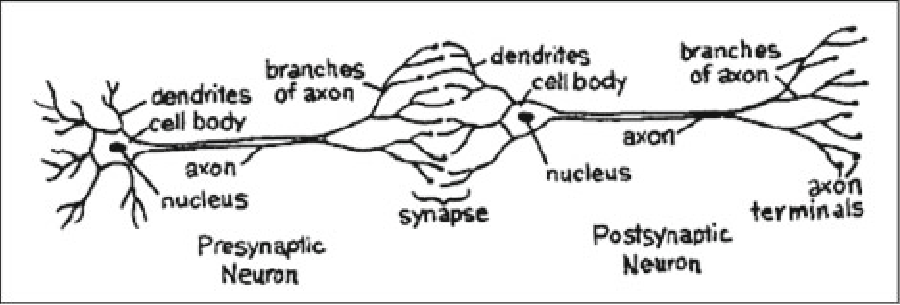
\includegraphics[width=\textwidth]{Sources/01-01_synapse.png}
    \label{Synapse}
    \caption{Synapse}
\end{subfigure}
\begin{subfigure}{0.25\textwidth}
    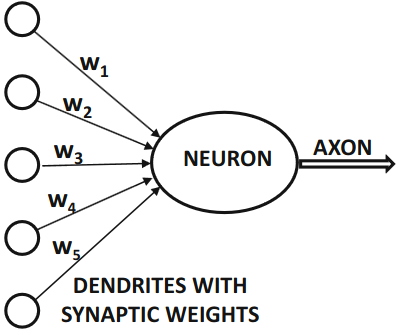
\includegraphics[width=\textwidth]{Sources/01-02_neuron.png}
    \label{Neuron}
    \caption{Neuron}
\end{subfigure}
\caption{Neural Networks and Deep Learning A Textbook, Charu C. Aggarwal
}
\end{figure}

Eines neuronales Netz besteht aus mindestens einem Neuron. Neuronen sind essentielle Bestandteile von neuralen Netzen. Sie nehmen Eingabedaten entgegen und wandeln diese 
in Ausgabedaten um. Neben den Eingabedaten werden auch Weight-Parameter übergeben, welche die zu berechnenden Werte beinflussen. Das eigenliche \enquote{Lernen} erfolgt durch diesen 
Einfluss.
\subsection{Arten von Neuronen}\label{subsec:neuronen:arten_von_neuronen}
  TEXT FOLGT... 
\newpage
\subsection{Funktionsweise}\label{subsec:neuronen:funktionsweise}
  %\input{}
  TEXT FOLGT... 
 

\newpage
\subsubsection{Aktivierungsfunktion}\label{subsec:neuronen:aktivierungsfunktion}
  Aktivierungsfunktionen ermöglichen den Neuronen nicht-lineare Outputs zu produzieren. Außerdem wird durch diese Funktionen entschieden, 
welche Neuronen aktiviert werden und wie die Inputs gewichtet werden. Zur Notation von Aktivierungsfunktion nutzen wir $\Phi$.
$$\hat{y} = \Phi(\overline{W} \cdot \overline{X})$$
\paragraph{Lineare Aktivierung}
Die simpelste Aktivierungsfunktion $\Phi(\cdot)$ ist die lineare Aktivierung. Sie bietet keine nicht linearität. Sie wird oft in Output Nodes
verwendet, wenn das Ziel ein reeler Wert ist.
$$\Phi(v) = v$$
\paragraph{Nicht lineare Aktivierung}
In den frühen Tagen der Entwicklung von neuralen Netzen wurden sign, sigmoid und hyperbolic tangent Funktionen genutzt.
\subparagraph{Sign Aktivierung}
Die sign Funktion generiert nur binäre \{-1,+1\} Ausgaben. Aufgrund der Nichtstätigkeit der Funktion, können beim Trainieren keine Loss-Funktionen verwendet werden.
$$\Phi(v) = \text{sign}(v)$$
\subparagraph{Sigmoid Aktivierung}
Die Sigmoid Funktion generiert Werte zwischen 0 und 1. Sie eignet sich deshalb für Rechnungen die als Wahrscheinlichkeiten interpetiert werden sollen.
$$\Phi(v) = \frac{1}{1 + e^{-v}}$$
\subparagraph{Tanh Aktivierung}
Der Graph der Tanh Funktion hat eine ähneliche Form wie die der Sigmoid Funktion. Sie unterscheidet sich jedoch in der Skalierung, denn ihre Wertebereich liegt zwischen -1 und 1.
$$\Phi(v) = \frac{e^{2v} - 1}{e^{2v} + 1}$$
Die Tanh Funktion lässt sich auch durch die Sigmoid Funktion darstellen.
$$\text{tanh}(v) = 2 \cdot \text{sigmoid}(2v) - 1$$
Wenn die Ausgabe der Berechnung postitiv sowie negativ sein kann, ist die tanh Funktion der sigmoid Funktion vorzuziehen. Außerdem ist es einfacher zu trainieren, weil die Funktion Mittelwertzentriert
und der Gradient größer ist.

\paragraph{Piecewise lineare Aktivierung}
Historisch wurden die Sigmoid und Tanh Funktion zur Einführung von Nichtliniearität genutzt. Heutzutage sind piecewise linear activation Funktionen (Stückweise Linear) beliebter, weil diese das Trainieren 
von mehrschichtigen neuronalen Netzen einfacher machen.
\subparagraph{ReLU}
TODO\\
$$\Phi(v) = \text{max}\{v,0\}$$
\subparagraph{hard tanh Aktivierung}
TODO\\
$$\Phi(v) = \text{max}\{\text{min}[v,1],-1\}$$

\begin{figure}[htbp]
    \centering
    \begin{subfigure}{0.3\textwidth}
      \centering
      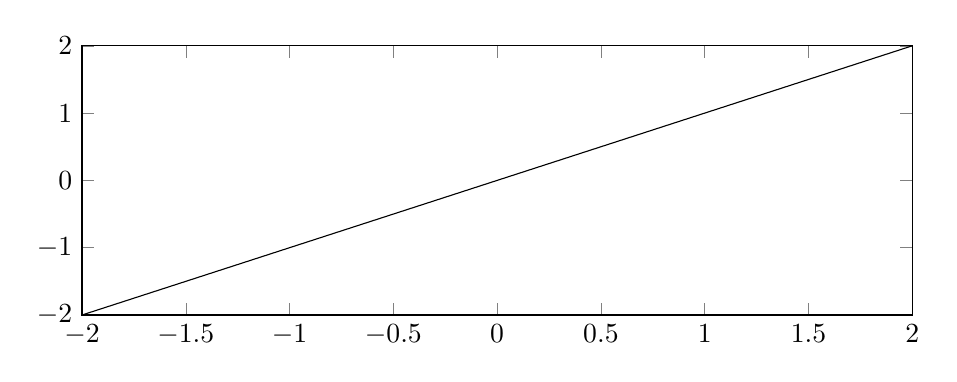
\begin{tikzpicture}
        \begin{axis}[
          width=\textwidth,
          height=5cm,
          xmin=-2,
          xmax=2,
          ymin=-2,
          ymax=2
        ]
          \addplot[black, domain=-2:2, samples=100] {x};
        \end{axis}
      \end{tikzpicture}
      \caption{Linear}
      \label{fig:plot1}
    \end{subfigure}
    \hfill
    \begin{subfigure}{0.3\textwidth}
        \centering
        \begin{tikzpicture}
          \begin{axis}[
            width=\textwidth,
            height=5cm,
            xmin=-2,
            xmax=2,
            ymin=-1.1,
            ymax=1.1,
            samples=100,
            xtick={-2,-1,0,1,2},
            ytick={-1,0,1},
            clip=false
          ]
            % Plot the sign function
            \addplot[black, thick, mark=none, domain=-2:0] {-1};
            \addplot[black, thick, mark=none, domain=0:2] {1};
            \draw (axis cs:0,-1) -- (axis cs:0,1);
          \end{axis}
        \end{tikzpicture}
        \caption{Sign Function}
        \label{fig:plot2}
      \end{subfigure}
    \hfill
    \begin{subfigure}{0.3\textwidth}
      \centering
      \begin{tikzpicture}
        \begin{axis}[
          width=\textwidth,
          height=5cm,
          xmin=-15,
          xmax=15,
          ymin=-1,
          ymax=1.1
        ]
          % Plot 3 data and settings
          \addplot[black, domain=-15:15, samples=100] {1/(1 + exp(-x))};
        \end{axis}
      \end{tikzpicture}
      \caption{Sigmoid}
      \label{fig:plot3}
    \end{subfigure}
  
    \medskip
  
    \begin{subfigure}{0.3\textwidth}
      \centering
      \begin{tikzpicture}
        \begin{axis}[
          width=\textwidth,
          height=5cm,
          xmin=-6.5,
          xmax=6.5,
          ymin=-1.1,
          ymax=1.1
        ]
          % Plot 4 data and settings
          \addplot[black, domain=-6.5:6.5, samples=100] {(exp(2*x)-1)/(exp(2*x)+1)};
        \end{axis}
      \end{tikzpicture}
      \caption{Tanh}
      \label{fig:plot4}
    \end{subfigure}
    \hfill
    \begin{subfigure}{0.3\textwidth}
      \centering
      \begin{tikzpicture}
        \begin{axis}[
            width=\textwidth,
            height=5cm,
            xmin=-2,
            xmax=2,
            ymin=-1.1,
            ymax=1.1
        ]
          % Plot 5 data and settings
          \addplot[black, domain=-2:2, samples=100] {max(x,0)};
        \end{axis}
      \end{tikzpicture}
      \caption{ReLU}
      \label{fig:plot5}
    \end{subfigure}
    \hfill
    \begin{subfigure}{0.3\textwidth}
      \centering
      \begin{tikzpicture}
        \begin{axis}[
            width=\textwidth,
            height=5cm,
            xmin=-2,
            xmax=2,
            ymin=-1.1,
            ymax=1.1
        ]
          % Plot 6 data and settings
          \addplot[black, domain=-2:2, samples=100] {max(min(x,1),-1)};
        \end{axis}
      \end{tikzpicture}
      \caption{Hard Tanh}
      \label{fig:plot6}
    \end{subfigure}
  
    \caption{Aktivierungsfunktionen}
    \label{fig:grid}
  \end{figure}
  
  TEXT FOLGT... 


\newpage
\subsubsection{Schichtenmodell}\label{subsec:neuronen:schichtenmodell}
  %\input{}
  TEXT FOLGT... 

\subsubsection{Loss-Function}

\newpage 
\subsection{Wie sind Neuronen miteinander verknüpft}\label{subsec:neuronen:verknuepfung_neuronen}  
%\input{}
Hier sollen die Weights erklärt werden

\subsubsection{Weights}\label{Weights}
  %\input{}
  TEXT FOLGT... 

\subsection{Fehler / Backpropagation Einführung}\label{subsec:neuronen:fehler_backpropagation}
Nur eine sehr knappe Einführung, da eigenes Kapitel für dieses Thema reserviert

